\section{ASPに基づくCAFE問題ソルバー}

開発したCAFE問題ソルバーの構成を図\ref{fig:system}に示す.
CAFE問題ソルバーでは,OVMで表現されたCAFE問題のインスタンスを
ASPファクト形式に変換した後,CAFE問題の制約のASP符号化と結合し,
高速ASPソルバーを用いて解を求める.

本節では,インスタンスのASPファクト形式による表現方法を説明し,
次に,制約の基本的なASP符号化と,その問題点を改良した符号化を提案する.
%以降では前者を基本符号化,後者を改良符号化と呼ぶ.

\begin{figure}[tb]
 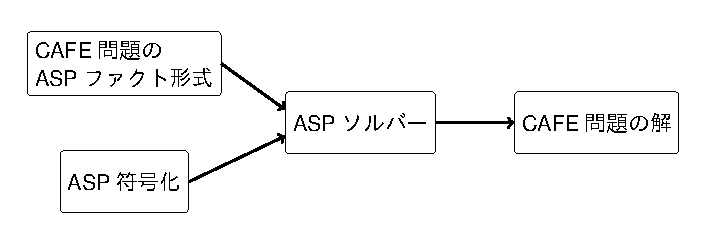
\includegraphics [width=\linewidth]{images/system.eps}
 \caption{CAFE問題ソルバーのシステム概要}
 \label{fig:system}
\end{figure}

\subsection{インスタンスのASPファクト形式}
\lstinputlisting[float=tb,caption={%
インスタンスのASPファクト表現(一部)},%
captionpos=b,frame=single,label=code:ovm2.lp,%
numbers=left,%
breaklines=true,%
columns=fullflexible,keepspaces=true,%
xrightmargin=0zw,% 
xleftmargin=3zw,% 
basicstyle=\ttfamily\scriptsize]{codes/ovm2.lp} 

コード\ref{code:ovm2.lp}は,図\ref{fig:ovm_example}のCAFE問題の
インスタンスの一部をASPファクト形式で表現したものである.

1行目ではタイプ\code{Drive\_Type}を定義している.
2,3行目ではオプション\code{2WD}と\code{4WD}を定義しており,
どちらもタイプ\code{Drive\_Type}に付随するオプションで,
IWRはそれぞれ\code{125}, \code{200}であることを表している.
5行目ではタイプ\code{Drive_Type}が必須であることを表している.
7行目はオプション\code{STD}がオプション\code{16_inch_Tire}を要求することを,
8行目はオプション\code{V4}がオプション\code{10AT}を排除することを意味する.
11行目で3つの装備仕様を求めるように指定している.




\subsection{基本符号化}
\lstinputlisting[float=tb,caption={%
CAFE問題のASP符号化},%
captionpos=b,frame=single,label=code:basic1.lp,%
numbers=left,%
breaklines=true,%
columns=fullflexible,keepspaces=true,%
xrightmargin=0zw,% 
xleftmargin=3zw,% 
basicstyle=\ttfamily\scriptsize]{codes/basic1.lp} 

コード\ref{code:basic1.lp}にCAFE問題の制約のASP符号化(基本符号化)を示す.
2行目は,CAFE基準値として変数\code{t}に整数90を代入している.変数\code{t}の値は
ソルバー使用時にオプションを加えることで,任意の値に変更することができる.

アトム\code{vp(VP,G)}, \code{v(V,G)}は,グループ\code{G}で
それぞれタイプ\code{VP},オプション\code{V}が装備されることを意味する.
%
4行目は,任意のタイプ\code{VP},任意のグループ\code{G}に対してタイプの解候補となる
\code{vp(VP,G)}を導入し,個数制約を用いてグループ\code{G}がタイプ\code{VP}を
装備するか否かの選択をするということを表している.
%
5行目は,一貫性制約を用いて必須であるタイプは必ず装備しなければならないという制約を表している.
%
6行目は,グループ\code{G}でタイプ\code{VP}が装備されるとき,
オプションの解候補となる\code{v(V,G)}を導入し,
個数制約を用いてタイプ\code{VP}に付随するオプションの中で装備するオプションの数を
ちょうど1つに制限している.


9〜12行目は燃費制約を表している.
9行目は重み付き個数制約を用いて,任意のグループ\code{G}に対して,
装備されるオプション\code{V}の\code{IWR}の和を変数\code{S}に代入し
アトム\code{iwr(S,G)}を生成する.このアトム\code{iwr(S,G)}は,
グループ\code{G}の装備仕様のIWRの和が\code{S}であることを表している.
%
10行目は,任意のグループ\code{G}と任意のIWRの和\code{S},任意の燃費\code{FE}に対して,
\code{iwr(S,G)}かつ\code{fe\_map(S,FE)}ならばアトム\code{fe(FE,G)}を生成する.
このアトム\code{fe(FE,G)}は,グループ\code{G}の装備仕様の燃費が値\code{FE}
であることを表している.
%
11行目は,任意のグループ\code{G}と,任意のIWR値の和\code{S},任意の販売台数\code{SV}
に対して,\code{S}に最も近い5の倍数\code{S1}を求める計算をし,\code{iwr(S,G)}かつ
\code{sv\_map(S1,SV)}ならば,アトム\code{sv(SV,G)}を生成する.
このアトム\code{sv(SV,G)}は,グループ\code{G}の装備仕様の販売台数が値\code{SV}
であることを表している.
%グループGのIWR値の和と燃費,販売台数のテーブルから,
%各装備仕様の燃費と販売台数を求めるためのルールで,
%アトムfe(FE,G), sv(SV,G)はそれぞれ,グループGの燃費がFE,
%販売台数がSVであることを表している.
%ただし,販売台数のテーブルではIWR値が5刻みになっているため,近似の値を取る.
12行目は,「販売台数を加味した全体の平均燃費が基準値\code{t}以上でなければならない」
という燃費制約を表している.第2章の燃費制約の式を変形すると,以下のようになる.
\vspace{1em}
\begin{displaymath}
 (FE_{1} - t) \times SV_{1} + (FE_{2} - t) \times SV_{2} + (FE_{3} - t)
 \times SV_{3} \geq 0
\end{displaymath}
\\
つまり,すべてのグループの\code{(FE - t)*SV}の和が0以上でなければならないという制約を,
一貫性制約と重み付き個数制約を用いて燃費制約を表現している.




15〜17行目は一貫性制約を用いて要求制約を表している.
15行目は,任意のオプション\code{V},任意のグループ\code{G}に対して,
\code{require\_v\_v(V,W)}かつ\code{v(V,G)}ならば,アトム\code{v(W,G)}は
真であることを意味する.
16, 17行目は,同様にして,タイプによるオプションの要求,オプションによるタイプの要求を
記述している.
16, 17行目は一貫性制約を用いて排他制約を表している.
%10行目は,グループ\code{G}がオプション\code{V}を装備するとき,
%オプション\code{V}がオプション\code{W}を要求するならば,
%オプション\code{W}も装備しなければならないということを意味する.


21行目は,目的関数である全体の販売台数の最大化を行っている.




\subsection{ASP符号化の改良}
\lstinputlisting[float=tb,caption={%
改良符号化の一部},%
captionpos=b,frame=single,label=code:basic2.lp,%
numbers=left,%
breaklines=true,%
columns=fullflexible,keepspaces=true,%
xrightmargin=0zw,% 
xleftmargin=3zw,% 
basicstyle=\ttfamily\scriptsize]{codes/basic2.lp} 

コード\ref{code:basic1.lp}の基本符号化では,9行目のIWRの和の候補の生成時に
オプションの個数制約を考慮しておらず,一つもオプションを選択しない場合や,
すべてのオプションを選択した場合など,明らかに成立しないオプションの選択の仕方による
IWRの和まで候補として生成してしまう.そこで,IWRの和の上下限をより厳密にした改良符号化の
一部をコード\ref{code:basic2.lp}に示す.

改良符号化では,前処理としてIWRの和の上下限の計算を行う.上限をすべてのタイプでIWRが最大のオプションを選択した場合の和,下限を必須であるタイプのみでIWRが最小のオプションを選択した場合の和としている.この上下限の値でIWRの和の候補を求める範囲を制限している.
